\documentclass[10pt,a4paper]{article}
\usepackage{amsmath}
\usepackage[utf8]{vietnam}
\usepackage{amsfonts}
\usepackage{amssymb}
\usepackage{graphicx}
\usepackage{float}
\usepackage{multicol}
\usepackage{tkz-tab}
\usepackage{colortbl}
\usepackage[left=2cm,right=2cm,top=2cm,bottom=2cm]{geometry}
\setlength{\parindent}{0pt}
\begin{document}
\fontsize{18}{30}\selectfont
{\centering TRƯỜNG ĐẠI HỌC CÔNG NGHỆ THÔNG TIN \\
KHOA KHOA HỌC MÁY TÍNH \\
BÀI TẬP MÔN PHÂN TÍCH VÀ THIẾT KẾ THUẬT TOÁN
\par}
\vspace{0.5 cm}
\begin{center}
    \begin{figure}[htp]
     \centering
\includegraphics[scale=.3]{images/logo_uit.jpg} \\
    \end{figure}
    \vspace{1 cm}
    
    \par\noindent\rule{\textwidth}{0.5pt}
    \fontsize{14}{30}\selectfont
    {\centering \textbf{HOMEWORK \#03 \\
    ĐỘ PHỨC TẠP VÀ CÁC KÝ HIỆU TIỆM CẬN} \\
    }
    \par\noindent\rule{\textwidth}{0.5pt}
    
    \fontsize{14}{30}\selectfont
    \begin{tabbing}
    \hspace{2 in} \= \hspace{2 in} \= \kill

    Môn: \> Phân tích thiết kế thuật toán \\
    Lớp: \> CS112.N23.KHCL \\
    Giảng viên hướng dẫn: \> Huỳnh Thị Thanh Thương \\
    Nhóm thực hiện: \> Hồ Thị Khánh Hiền(Leader) - 21522057 \\
    \hspace{5.3 cm}Tống Trần Tiến Dũng - 21521983 \\
    \hspace{5.3 cm}Bùi Mạnh Hùng - 21522110 \\
    \end{tabbing}  

    \begin{center}
    \fontsize{14}{30}\selectfont
     TP Hồ Chí Minh,{\today}
    \end{center}
\end{center}
\newpage
\fontsize{13}{15}\selectfont
\tableofcontents
\newpage
%write table of contents without Index
%Ex: 
% Bài 1
\section*{Bài tập 1} 
\addcontentsline{toc}{section}{Bài tập 1}
\subsection*{a)}
Độ phức tạp: \\
- sử dụng để đánh giá tính hiệu quả về mặt không gian hoặc thời gian của thuật toán.\\
- phân loại cấp độ lớn, đánh giá cấp độ lớn ( khi n đủ lớn).\\
- Độ phức tạp không phải là một khái niệm khoa học, toán học\\
- biểu diễn thông qua hệ thống các kí hiệu tiệm cận $\Omega, \mathcal{O}, \theta$, liên quan đến chặn biên
\subsection*{b)}
\begin{figure}[H]
        \centering
        
\includegraphics[scale=0.75]{images/1b.png}
\end{figure}
Người ta thường không quan tâm đến bản thân thời gian thực hiện T(n) vì:
\begin{itemize}
    \item Trong thực tế, rất khó để tính T(n) chính xác
    \item Nếu tính được T(n) rồi thì có thể gặp khó khăn khác khi so sánh 2 hàm số với nhau
    \item Thời gian chính xác thực hiện T(n) phụ thuộc vào độ lớn của n
    \item Thời gian thực thi còn phụ thuộc vào tình trạng máy (thay đổi theo thời gian) => so sánh các thuật toán với nhau không chính xác
\end{itemize}
=> Khi nghiên cứu về thuật toán, người ta thường quan tâm đến bậc tăng trưởng chứ không phải là bản thân thời gian thực hiện T(n) (nhận định trên là đúng) 
\subsection*{c)Nói về ĐPT tức là đề cập tới các ký hiệu tiệm cận, mà có nhiều ký hiệu khác nhau. Vậy khi nào(trong trường hợp nào) thì nên dùng ký hiệu nào ?}
\text{Có 3 ký hiệu tiệm cận thường dùng, đó là: }
\begin{itemize}
    \item $\mathcal{O}$(big oh): khi muốn đánh giá độ phức tạp của giải thuật trong trường hợp xấu nhất
    \subitem VD: $f(n) = 100n+5 \in \mathcal{O}(n)$
    \item $\Omega$(big omega): khi muốn đánh giá độ phức tạp của giải thuật trong trường hợp tốt nhất
    \subitem VD: $f(n) = n^3 \in \Omega(n^2)$
    \item $\Theta$(big theta): khi muốn đánh giá độ phức tạp của giải thuật trong trường hợp trung bình
    \subitem VD: $f(n) = \frac{1}{2}n(n-1) \in \Theta(n^2)$
\end{itemize}
% Bài 2
\section*{Bài tập 2} 
\addcontentsline{toc}{section}{Bài tập 2}
\textbf{For each function f(n) and time t in the following table, determine the largest size n of a problem that can be solved in time t, assuming that the algorithm to solve the problem takes f(n) microseconds}\\
\begin{table}[H]
    \centering
    \begin{tabular}[c]{|p{0.85cm}|p{2cm}|p{2cm}|p{2cm}|p{2cm}|p{2cm}|p{2cm}|p{2.3cm}|}\hline
     \rowcolor[rgb]{0, .60, .800}& 1 second&1 minute&1 hour&1 day&1 month&1 year&1 century \tabularnewline\hline
    $\log{n}$  & $2{10^{3}}$ & $2{6.10^{4}}$ & $2{36.10^{5}}$ & $2{864.10^{5}}$ & $2{2592.10^{6}}$ & $2{31104.10^{7}}$ & $2{31104.10^{9}}$ \tabularnewline\hline
    $\sqrt{n}$ & $10^6$ & $36.10^8$ & $1926.10^{10}$ & $\approx 7460.10^{12}$ & $\approx 6718.10^{15}$ & $\approx 8951.10^{20}$ & $\approx 8951.10^{24}$ \tabularnewline\hline
    n & $10^{3}$ & $6.10^{4}$ & $36.10^{5}$ & $864.10^{5}$ & $2592.10^{6}$ & $31104.10^{7}$ & $31104.10^{9}$ \tabularnewline\hline
    $n\log{n}$ & 62746 & 2801417 & 133378058 & 2755147513 & 71870856404 & 797633893349 & 68610956750570 \tabularnewline\hline
    $n^2$  & 1000 & 7745 & 60000 & 293938 & 1609968 & 5615692 & 56156922 \tabularnewline\hline
    $n^3$ & 100 & 391 & 1532 & 4420 & 13736 & 31593 & 146645 \tabularnewline\hline
    $2^n$ & 19 & 25 & 31 & 36 & 41 & 44 & 51 \tabularnewline\hline
    n! & 9 & 11 & 12 & 13 & 15 & 16 & 17 \tabularnewline\hline
    \end{tabular}
\end{table}
\textbf{Giải thích:}\\
Theo giả thiết bài toán, giải thuật xử lý trong f(n) (microseconds) hay f(n) = t(microseconds)\\
Với mỗi $f(n)$ ta thử từng trường hợp n để tìm giá trị n lớn nhất thỏa mãn, theo các đoạn code sau:
\begin{itemize}
    \item $logn, \sqrt{n}, n: $
     \begin{figure}[H]
        \centering
        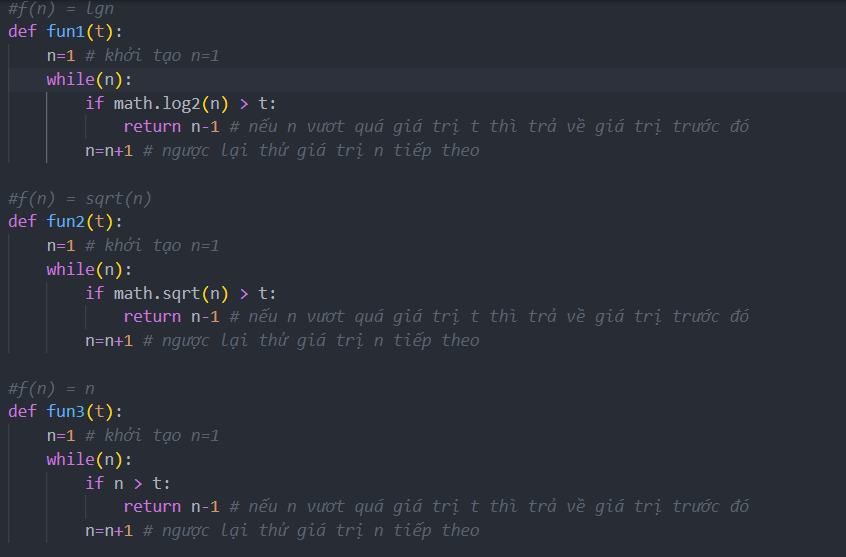
\includegraphics[scale=0.75]{images/2.1.png}
    \end{figure}
     \begin{figure}[H]
        \centering
        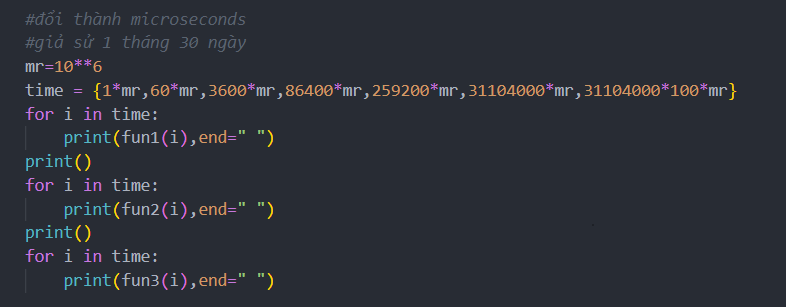
\includegraphics[scale=0.75]{images/2.1.b.png}
    \end{figure}
    \item $nlogn, n^2, n^3: $
     \begin{figure}[H]
        \centering
        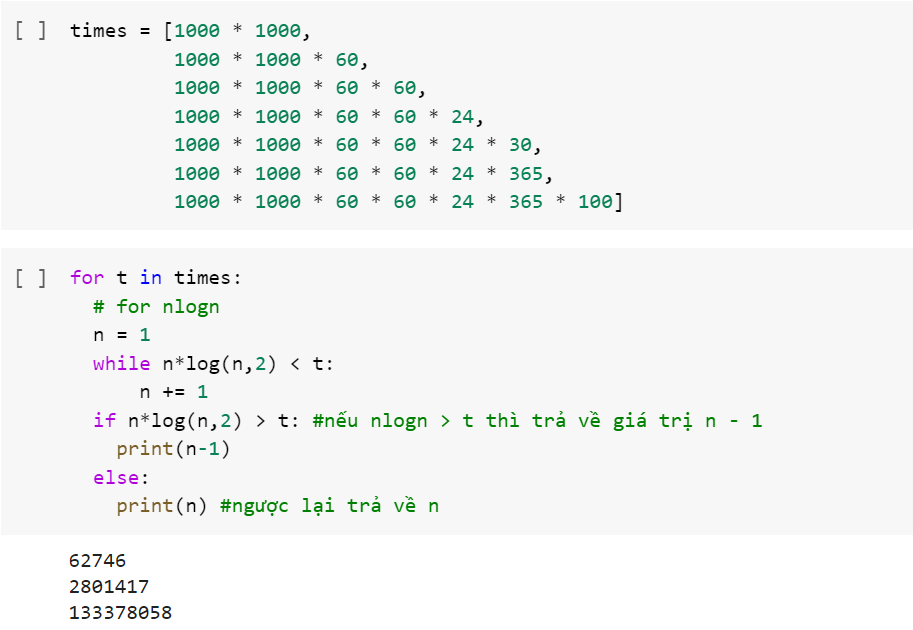
\includegraphics[scale=0.75]{images/nlogn.png}
    \end{figure}
     \begin{figure}[H]
        \centering
        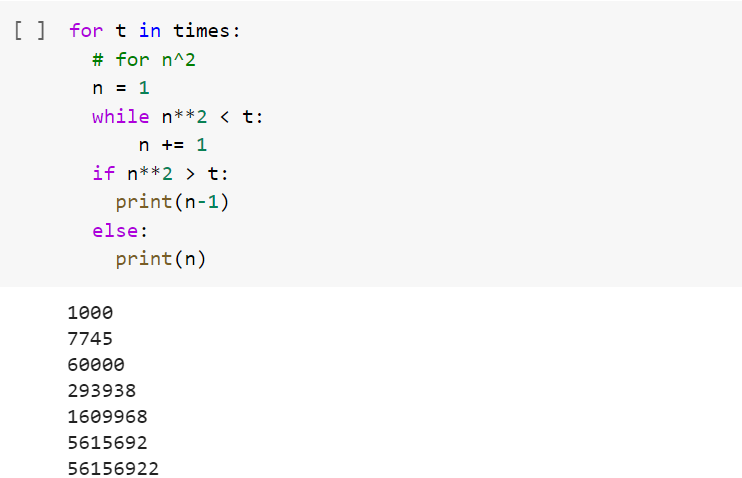
\includegraphics[scale=0.9]{images/n2.png}
        \centering
        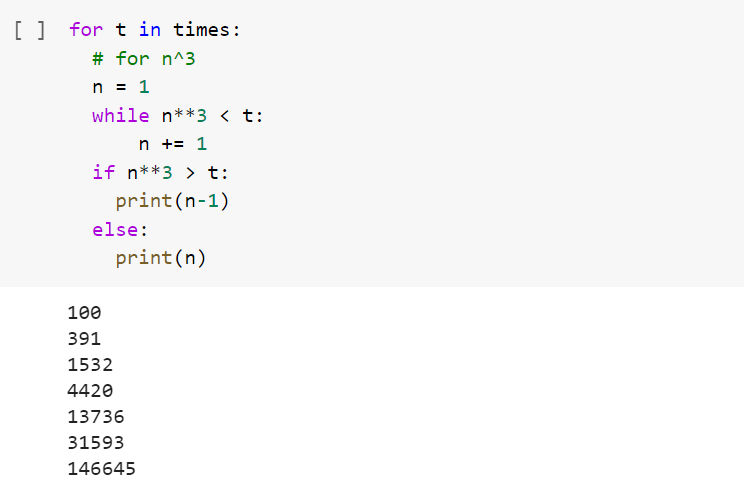
\includegraphics[scale=0.9]
        {images/n3.png}
    \end{figure}
    \item $2^n, n!: $
    \begin{figure}[H]
        \centering
        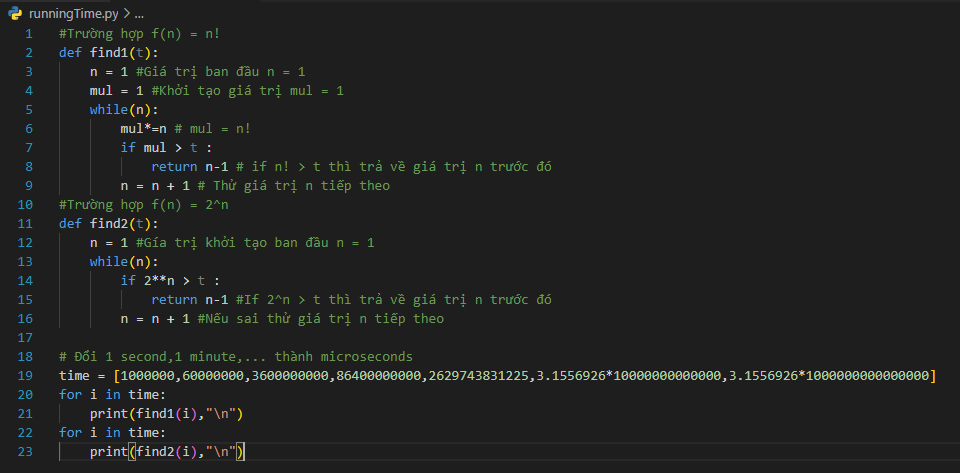
\includegraphics[scale=0.7]{images/runningtime.png}
    \end{figure}
\end{itemize}


% Bài 3
\section*{Bài tập 3} 
\addcontentsline{toc}{section}{Bài tập 3}
\subsection*{a)}
\begin{figure}[H]
    \centering
    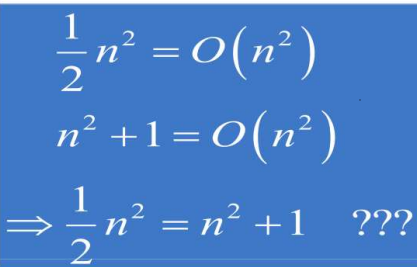
\includegraphics[scale=0.8]{images/3a.png}
\end{figure}
Phép suy ra bên trên là sai, dấu bằng "=" ở đây chỉ về mặt hình thức, chính xác hơn ở đây là dấu thuộc "$\in$".\\
Có nghĩa là 2 hàm trên đều thuộc tập hợp \{$t(n):  \exists c \in R^+,\exists n_0\in N,\forall n \geq n_0,t(n)\leq cn^2$\}\\
\subsection*{b)}
\begin{figure}[H]
    \centering
    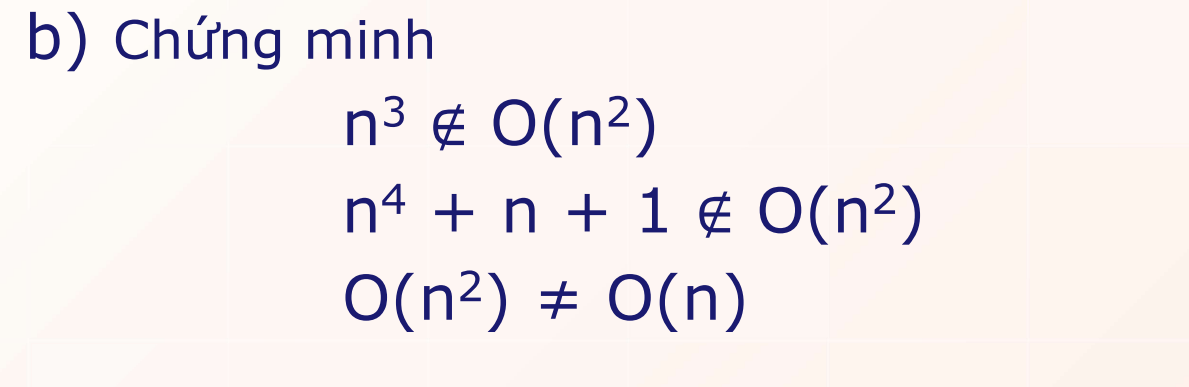
\includegraphics[scale=0.8]{images/3b.png}
\end{figure}
\begin{itemize}
    \item Giả sử $n^3 \in \mathcal{O}(n^2) \Rightarrow \exists c \in \mathbb{R^+} ,\exists n_0 \in \mathbb{N}$ sao cho: $n^3 \leq cn^2$ ($\forall n \geq n_0) \Rightarrow n \leq c$\\
    Với n = c+1 thì $n \leq c $ sai $\Rightarrow n \notin \mathcal{O}(n^2)$ (đccm)
    \item Giả sử $n^4 + n + 1 \in \mathcal{O}(n^2) \Rightarrow \exists c \in \mathbb{R^+} ,\exists n_0 \in \mathbb{N}$ sao cho: $n^4 + n + 1 \leq cn^2$ ($\forall n \geq n_0) \Rightarrow n^2 + 1/n + 1/n^2 \leq c$\\
    Chọn n = 1/c $\Rightarrow \frac{1}{c^2} + c + c^2 \leq c \Rightarrow \frac{1 + c^4}{c^2} \leq 0 \Rightarrow 1 + c^4 \leq 0 \Rightarrow c^4 \leq -1$\\
    Mà c>0 => $c^4 > 0 \forall c \Rightarrow$ không tồn tại c để $n^4 + n + 1 \leq cn^2\\ \Rightarrow n^4 + n + 1 \notin \mathcal{O}(n^2)$ (đccm)
    \item Để CM $\mathcal{O}(n^2) \ne \mathcal{O}(n)$ tìm f(n) $\in \mathcal{O}(n^2)$ nhưng f(n) $\notin \mathcal{O}(n)$\\
    Chọn f(n) = $n^2$\\
    f(n) $\in \mathcal{O}(n^2)$ với $c_1 = 1, n_0$ =1 \\Giả sử $n^2 \in \mathcal{O}(n) \Rightarrow \exists c_1 \in \mathbb{R^+} ,\exists n_1 \in \mathbb{N}$ sao cho: $n^2 \leq c_1n$ $(\forall n \geq n_1)\Rightarrow n \leq c_1$\\
    Với n = $c_1 + 1$ thì $n \leq c_1$ sai $\Rightarrow n^2 \notin \mathcal{O}(n)$\\
    $\Rightarrow \mathcal{O}(n^2) \not\subset \mathcal{O}(n)\Rightarrow \mathcal{O}(n^2) \ne  \mathcal{O}(n)$ (đccm)
\end{itemize}
\subsection*{c)}
\begin{figure}[H]
    \centering
    
\includegraphics[scale=0.8]{images/3c.png}
\end{figure}
\text{Ta có: }\\
$a_kn^k+a_{k-1}n^{k-1}+...+a_1n+a_0 \leq |a_k|n^k + |a_{k-1}|n^{k-1} + ...+|a_1|n+|a_0|$ $\forall n \geq 1$ \\
$=> T(n) \leq (|a_k| + |a_{k-1}| + ...+|a_1| + |a_0|)n^k$ $\forall n \geq 1$ \\
Chọn $c = |a_k| + |a_{k-1}| + ...+|a_1| + |a_0| $,$n_0 = 1$, theo định nghĩa của Big Oh, ta có: $T(n) = \mathcal{O}(n^k)$(đccm)
% Bai 4
\section*{Bài tập 4} 
\addcontentsline{toc}{section}{Bài tập 4}
\subsection*{Group 1)}
\begin{figure}[H]
    \centering
    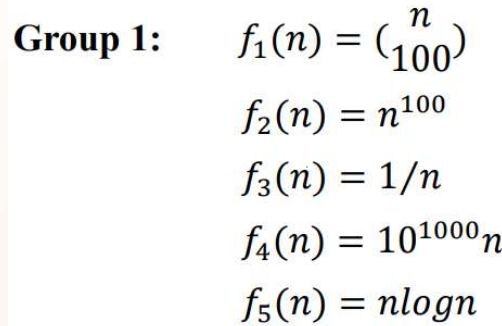
\includegraphics[scale=.8]{images/4.1.png}
\end{figure}
$f_1(n) = C_n^100 = \frac{n!}{(n-100)!100!} = \mathcal{O}(n^{100})\\
f_2(n) =  \mathcal{O}(n^{100})\\
f_3(n) = \frac{1}{n} =  \mathcal{O}(n^{-1})\\
f_4(n) = 10^{1000}n = \mathcal{O}(n)\\
f_5(n) = nlogn = n.n^{\log_n{logn}} = \mathcal{O}(n^{1+c})$\\
Vậy $f_3(n) < f_4(n) \approx f_5(n) < f_1(n) \approx f_2(n)$
\subsection*{Group 2)}
\begin{figure}[H]
    \centering
    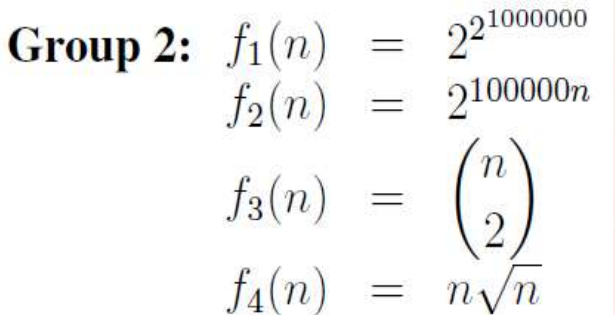
\includegraphics[scale=.8]{images/4.2.png}
\end{figure}
$f_1(n) = 2^{2^{1000000}} = \mathcal{O}(1)\\
f_2(n) = 2^{100000n} = \mathcal{O}(2^n)\\
f_3(n) = C_n^2 =\frac{n!}{(n-2)!2!} = \mathcal{O}(n^2)\\
f_4(n) = n\sqrt{n} = n^{3/2} = \mathcal{O}(n^{3/2})$\\
Vậy $f_1(n) < f_4(n) < f_3(n) < f_2(n)$
\subsection*{Group 3)}
\begin{figure}[H]
    \centering
    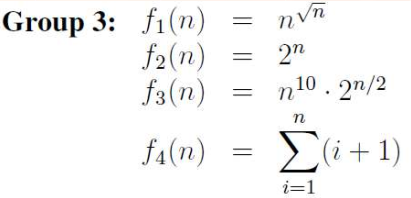
\includegraphics[scale=1]{images/4g3.png}
\end{figure}
\text{Ta thấy:}\\
$f_1(n) = n^{\sqrt{n}} = (2^{\log_2{n}})^{\sqrt{n}} = 2^{\sqrt{n}\log_2{n}} = 2^{\mathcal{O}(n^{c+1/2})}$ \text{với c > 0} \\
$f_2(n) = 2^n = 2^{\mathcal{O}(n)}$ \\
$f_3(n) = {n^{10}}{2^{\frac{n}{2}}} = {2^{10{\log_2{n}}}}{2^{\frac{n}{2}}} = 
2^{10{\log_2{n}} + \frac{n}{2}} = 2^{\mathcal{O}(n)}$\\
$f_4(n) = \sum_{i=1}^{n}(i+1) = \frac{n(n+1)}{2} = 2^{\log_2{\frac{n^2+n}{2}}} = 2^{\mathcal{O}(n^c)}$ \text{với c > 0} \\
Vậy $f_4(n) < f_1(n) < f_2(n) \approx f_3(n)$
\subsection*{Group 4)}
\begin{figure}[H]
    \centering
    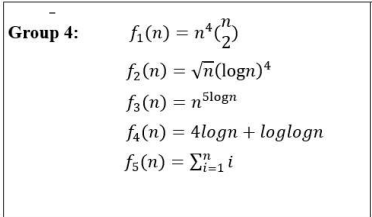
\includegraphics[scale=1]{images/4.4.png}
\end{figure}
$logn \in \mathcal{O}(n^c)$ với c có thể rất bé nhưng c >0\\
$f_1(n) = n^4.\frac{n!}{(n-2)!2!} = n^{\mathcal{O}(6)}\\
f_2(n) = n^{1/2}n^{4\log_n(logn)} = n^{\mathcal{O}(1/2 + 4c)}\\
f_3(n) =  n^{\mathcal{O}(logn )}\\
f_4(n) =  n^{\mathcal{O}(c)}\\
f_{5}(n) = 4^{n^{1/4}} = \frac{n(n-1)}{2} = n^{\mathcal{O}(2)}\\
$
Vậy $f_2(n) \approx f_4(n) < f_{1}(n) \approx f_5(n)  < f_3(n)$
\subsection*{Group 5)}
\begin{figure}[H]
    \centering
    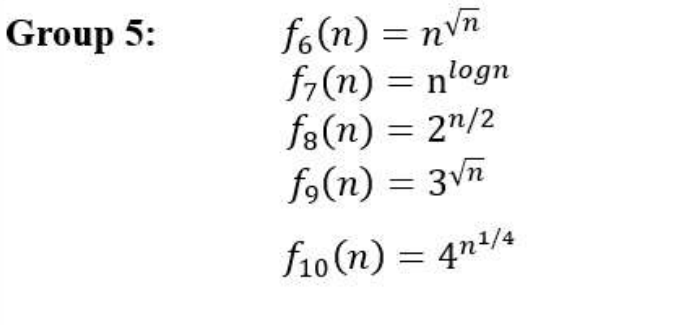
\includegraphics[scale=1]{images/4.5.png}
\end{figure}
$logn \in \mathcal{O}(n^c)$ với c có thể rất bé nhưng c >0\\
$f_6(n) = n^{\sqrt{n}} = (2^{logn})^{\sqrt{n}} = 2^{\sqrt{n}logn} = 2^{\mathcal{O}(\sqrt{n}n^c)} = 2^{\mathcal{O}(n^{1/2 + c})}\\
f_7(n) = n^{logn} = (2^{logn})^{logn} = 2^{\mathcal{O}(n^{2c})}\\
f_8(n) = 2^{n/2} =  2^{\mathcal{O}(n/2)}\\
f_9(n) = 3^{\sqrt{n}} = 2^{log3\sqrt{n}} = 2^{\mathcal{O}(n^{1/2})}\\
f_{10}(n) = 4^{n^{1/4}} = 2^{2n^{1/4}} = 2^{\mathcal{O}(n^{1/4})}\\
$
Vậy $f_7(n) < f_{10}(n) < f_9(n) \approx f_6(n) < f_8(n)$
\subsection*{Group 6)}
\begin{figure}[H]
    \centering
    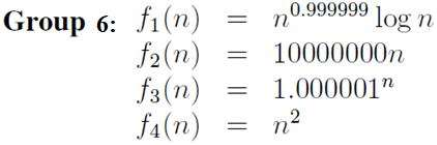
\includegraphics[scale=1]{images/4g6.png}
\end{figure}
\text{Ta thấy:}\\
$f_1(n) = n^{0.999999}\log{n} = \mathcal{O}(\log(n))$\\
$f_2(n) = 10000000n = \mathcal{O}(n)$ \\
$f_3(n) = 1,000001^n = \mathcal{O}(c^n)$\\
$f_4(n) = n^2 = \mathcal{O}(n^2)$\\
Vậy $f_1(n) < f_2(n) < f_4(n) < f_3(n)$
\subsection*{Group 7)}
\begin{figure}[H]
    \centering
    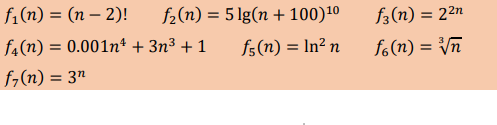
\includegraphics[scale=1]{images/4.7.png}
\end{figure}
\text{Ta thấy:}\\
$f_1(n) = \mathcal{O}(n!)$\\
$f_2(n) = 50log(n+100) = \mathcal{O}(n^c)$ \\
$f_3(n) = \mathcal{O}(c^n)$\\
$f_4(n) = \mathcal{O}(n^4)$\\
$f_5(n) = ln^22.log^2n =  \mathcal{O}(n^{2c})$\\
$f_6(n) =  \mathcal{O}(n^{1/3})$\\
$f_7(n) =  \mathcal{O}(c^n)$\\
Vậy $f_2(n) < f_5(n ) < f_6(n) < f_4(n) < f_7(n) < f_3(n) <f_1(n)$
% Bai 5
\section*{Bài tập 5} 
\addcontentsline{toc}{section}{Bài tập 5}
\subsection*{a) $\mathcal{O}(C) = \mathcal{O}(1)$ với C là hằng số}
\begin{itemize}
    \item $\mathcal{O}(C) \subset \mathcal{O}(1)\\$
    Chọn bất kỳ $f(n) \in \mathcal{O}(C) \Rightarrow \exists d \in \mathbb{R^+}$ $,\exists n_1 \in \mathbb{N}$ sao cho: $f(n) \leq dC$ $\forall(n \geq n_1)$ \\
    Chọn $k_1 = dC, n_3 = n_1 \Rightarrow f(n) \leq k_1.1$ $ (\forall n \geq n_3)$$\Rightarrow \mathcal{O}(C) \subset \mathcal{O}(1)$
     \item $\mathcal{O}(1) \subset \mathcal{O}(C)\\$
     Chọn bất kỳ $f(n) \in \mathcal{O}(1) \Rightarrow \exists e \in \mathbb{R^+}$ $,\exists n_2 \in \mathbb{N}$ sao cho: $f(n) \leq e.1$ $\forall(n \geq n_2)$ \\
    Chọn $k_2 = a/C, n_4 = n_2 \Rightarrow f(n) \leq k_2.C.1=k_2.C$ $ (\forall n \geq n_4)$$ \Rightarrow \mathcal{O}(1) \subset \mathcal{O}(C)$
\end{itemize}
$\Rightarrow \mathcal{O}(C) = \mathcal{O}(1)$ với C là hằng số (\textbf{đccm})
\subsection*{b) Nếu $f(n) \in \mathcal{O}(g(n))$ và $g(n) \in \mathcal{O}(h(n))$ thì $f(n) \in \mathcal{O}(h(n))$}
\text{Ta có: }
\begin{itemize}
    \item $f(n) \in \mathcal{O}(g(n))$ $=> \exists c_1 \in \mathbb{R^+}$ $,\exists n_1 \in \mathbb{N}$ $| f(n) \leq c_1g(n)$ $\forall n \geq n_1$
    \item $g(n) \in \mathcal{O}(h(n))$ $=> \exists c_2 \in \mathbb{R^+}$ $,\exists n_2 \in \mathbb{N}$ $| g(n) \leq c_2h(n)$ $\forall n \geq n_2$
\end{itemize}
$=> \forall n \geq max(n_1,n_2)$ thì $f(n) \leq c_1c_2h(n)$ \\
\text{Vậy, chọn $c=c_1c_2,$ $n_0 = max(n_1,n_2)$ => $f(n) \in \mathcal{O}(h(n))$\textbf{(đccm)}}
\subsection*{c) max\{f(n),g(n)\} = $\theta(f(n)+g(n))$}
giả sử: $f(n)\geq0$ và $g(n)\geq0$
,$\forall n \geq n_0$\\
ta thấy$ f(n) \leq max\{f(n),g(n)\} $ và $ g(n) \leq max\{f(n),g(n)\}  $\\
$\rightarrow f(n) + g(n) \leq 2max\{f(n),g(n)\}$\\
$\Leftrightarrow 1/2(f(n)+g(n))\leq max\{f(n),g(n)\} \leq f(n)+g(n)$\\
$c_1$ = $\frac{1}{2}$, $c_2$ = $1$\\
Dựa theo định nghĩa của Big-$\theta$
$\rightarrow max\{f(n),g(n)\} = \theta(f(n)+g(n))$\\

\subsection*{d)
If t(n)$\in \mathcal{O}(g(n))$ then g(n) $\in \Omega(t(n))$ }
t(n)$\in \mathcal{O}(g(n)) \Rightarrow \exists c \in \mathbb{R^+},\exists n_0 \in \mathbb{N}$ sao cho:$ t(n) \leq cg(n)$ $(\forall n \geq n_0) \\
\Rightarrow \frac{1}{c}t(n) \leq g(n)$ $(\forall n \geq n_0)$\\
Chọn d = 1/c, $n_1=n_0$ $\Rightarrow dt(n) \leq g(n)$ $(\forall n \geq n_1)$\\
Dựa theo định nghĩa của Big-$\Omega$ thì 
g(n) $\in \Omega(t(n))$ (\textbf{đccm})
\subsection*{e) $\Theta(\alpha g(n)) = \Theta(g(n))$, where $\alpha > 0$}
\textbf{Ta cần chứng minh $\Theta(\alpha g(n)) \subset \Theta(g(n))$} \\
\text{Xét một hàm số bất kỳ} $f(n) \in \Theta(\alpha g(n))$ \\
$=> \exists d_1,d_2 \in \mathbb{R^+}$ $,n_0 \in \mathbb{N}$ $ | d_1\alpha g(n) \leq f(n) \leq d_2\alpha g(n)$ $ \forall n \geq n_0$ \\
Chọn $k_1= d_1\alpha, k_2=d_2\alpha$ vì $\alpha > 0$ $=> k_1,k_2 \in \mathbb{R^+}$,ta có:\\
\centerline{$k_1g(n) \leq f(n) \leq k_2g(n)$ $\forall n \geq n_0$}
=>$f(n) \in \Theta(g(n))$ => $\Theta(\alpha g(n)) \subset \Theta(g(n))$ \textbf{(1)}\\

\textbf{Ta cần chứng minh $\Theta(g(n)) \subset \Theta(\alpha g(n))$} \\
\text{Xét một hàm số bất kỳ} $f(n) \in \Theta(g(n))$ \\
$=> \exists d_1,d_2 \in \mathbb{R^+}$ $,n_0 \in \mathbb{N}$ $ | d_1 g(n) \leq f(n) \leq d_2 g(n)$ $ \forall n \geq n_0$ \\
Chọn $k_1= \frac{d_1}{\alpha}, k_2=\frac{d_2}{\alpha}$ vì $\alpha > 0$ $=> k_1,k_2 \in \mathbb{R^+}$,ta có:\\
\centerline{$k_1\alpha g(n) \leq f(n) \leq k_2\alpha g(n)$ $\forall n \geq n_0$}
=>$f(n) \in \Theta(\alpha g(n))$ => $\Theta(g(n)) \subset \Theta(\alpha g(n))$ \textbf{(2)}\\
Từ \textbf{(1)} và \textbf{(2)} => $\Theta(\alpha g(n)) = \Theta(g(n))$, where $\alpha > 0$\\
\text{Vậy khẳng định trên là \textbf{đúng}}
\subsection*{f) $\theta(g(n)) = \mathcal{O}(g(n)) \cap \Omega(g(n)) $}
\textbf{Chứng minh: $\theta(g(n)) \subset \mathcal{O}(g(n)) \cap \Omega(g(n))$}\\
giả sử: $\forall f(n) \in \theta(g(n))$\\
$\exists c_1,c_2\in R^+, \exists n_0 \in N \rightarrow c_1g(n) \leq f(n) \leq c_2g(n) \forall n \geq n_0$\\
suy ra : \\
   +> $\forall n \geq n_0,  c_1g(n) \leq f(n) \Rightarrow f(n) \in \Omega(g(n))$\\
   +> $\forall n \geq n_0,   f(n) \leq c_2g(n) \Rightarrow f(n) \in \mathcal{O}(g(n))$\\
   $\Rightarrow f(n) \in \mathcal{O}(g(n)) \cap \Omega(g(n))$\\
   vậy $\forall f(n) \in \theta(g(n)), f(n) \in \mathcal{O}(g(n)) \cap \Omega(g(n))$\\
   $\Rightarrow \theta(g(n)) \subset \mathcal{O}(g(n)) \cap \Omega(g(n))$ (1)\\
\textbf{Chứng minh: $\mathcal{O}(g(n)) \cap \Omega(g(n))$} $\subset \theta(g(n))$\\
giả sử: $\forall f(n) \in \mathcal{O}(g(n)) \cap \Omega(g(n))$\\
suy ra : \\
   +> $\exists c_1 \in R^+, \exists n_0 \in N \rightarrow f(n) \leq c_1g(n) \forall n \geq n_0$\\
   +> $\exists c_2 \in R^+, \exists n_1 \in N \rightarrow f(n) \geq c_2g(n) \forall n \geq n_1$\\
   $\rightarrow c_2g(n) \leq f(n) \leq c_1g(n)  \forall n \geq max\{n_0,n_2\}$\\
    $\Rightarrow f(n) \in \theta(g(n))$\\
   vậy $\forall f(n) \in \mathcal{O}(g(n)) \cap \Omega(g(n)), f(n) \in \theta(g(n))$\\
   $\Rightarrow \mathcal{O}(g(n)) \cap \Omega(g(n))$ $\subset \theta(g(n))$ (2)\\
từ (1) và (2) $\Rightarrow \theta(g(n)) = \mathcal{O}(g(n)) \cap \Omega(g(n)) $ 

% Bài 6
\section*{Bài tập 6: Các khẳng định bên dưới là đúng hay sai? Vì sao?} 
\addcontentsline{toc}{section}{Bài tập 6: Các khẳng định bên dưới là đúng hay sai? Vì sao?}
\subsection*{a) Nếu $f(n) = \Theta(g(n))$ và $g(n) = \Theta(h(n))$, thì $h(n) = \Theta(f(n))$}
Có:
\begin{itemize}
    \item $f(n) = \Theta(g(n)) \Rightarrow f(n) = \mathcal{O}(g(n))$ và $g(n) = \mathcal{O}(f(n))$
    \item $g(n) = \Theta(h(n)) \Rightarrow g(n) = \mathcal{O}(h(n))$ và $h(n) = \mathcal{O}(g(n))$
\end{itemize}
Cần CM: $f(n) = \mathcal{O}(h(n))$ và $h(n) = \mathcal{O}(f(n))$
\begin{itemize}
    \item $f(n) = \mathcal{O}(h(n))$\\
    $f(n) = \mathcal{O}(g(n)) \Rightarrow \exists c_1 \in \mathbb{R^+}, n_1 \in \mathbb{N}$ sao cho: $f(n) \leq c_1g(n)\\ \Rightarrow \frac{1}{c_1}f(n) \leq g(n)$ $\forall n \geq n_1$ (1)\\
    $g(n) = \mathcal{O}(h(n)) \Rightarrow \exists c_2 \in \mathbb{R^+}, n_2 \in \mathbb{N}$ sao cho: $g(n) \leq c_2h(n)$ $\forall n \geq n_2$ (2)\\
    Từ (1) và (2) $\Rightarrow \frac{1}{c_1}f(n) \leq c_2h(n) \Rightarrow f(n) \leq c_1c_2h(n)$ $\forall n \geq n_1, n \geq n_2$\\
    Chọn a = $c_1c_2, n_3 =$ max($n_1, n_2$) $\Rightarrow f(n) \leq ah(n)$  $\forall n \geq n_3 \Rightarrow f(n) = \mathcal{O}(h(n))$
    \item $h(n) = \mathcal{O}(f(n))$\\
    $g(n) = \mathcal{O}(f(n)) \Rightarrow \exists c_3 \in \mathbb{R^+}, n_4 \in \mathbb{N}$ sao cho: $g(n) \leq c_3f(n)\\$ $\forall n \geq n_4$ (3)\\
    $h(n) = \mathcal{O}(g(n)) \Rightarrow \exists c_4 \in \mathbb{R^+}, n_5 \in \mathbb{N}$ sao cho: $g(n) \leq c_4h(n) \\ \Rightarrow \frac{1}{c_4}g(n) \leq h(n)$ $\forall n \geq n_5$(4)\\
    Từ (3) và (4) $\Rightarrow \frac{1}{c_4}h(n) \leq c_3f(n) \Rightarrow h(n) \leq c_3c_4f(n)$ $\forall n \geq n_4, n \geq n_5$\\
    Chọn b = $c_3c_4, n_6 =$ max($n_3, n_4$) $\Rightarrow hf(n) \leq bf(n)$  $\forall n \geq n_6 \Rightarrow h(n) = \mathcal{O}(f(n))$
\end{itemize}
$\Rightarrow h(n) = \Theta(f(n))$ \\
\text{Vậy khẳng định trên là \textbf{đúng}}
\subsection*{b) Nếu $f(n) = \mathcal{O}(g(n))$ và $g(n) = \mathcal{O}(h(n))$, thì $h(n) = \Omega(f(n))$}
Từ giả thiết:
\begin{itemize}
    \item $f(n)=\Theta(g(n))$$=> \exists c_1 \in \mathbb{R^+}, n_1 \in \mathbb{N}$ $| f(n) \leq c_1g(n)$ $\forall n \geq n_1$
    \item $g(n)=\Theta(h(n))$$=> \exists c_2 \in \mathbb{R^+}, n_2 \in \mathbb{N}$ $| g(n) \leq c_2h(n)$ $\forall n \geq n_2$
\end{itemize}
=> Với $n_0 = max(n_1,n_2) => f(n) \leq c_1c_2h(n)$ $\forall n \geq n_0$ \\
=> Chọn $n_0 = max(n_1,n_2)$ và $c_0 = c_1c_2$ thì $f(n) = \mathcal{O}(h(n))$ hay $h(n) = \Omega(f(n))$ \textbf{(đccm)}
\subsection*{c) Nếu f(n) = $\mathcal{O}(g(n))$ và g(n) = $\mathcal{O}(f(n))$ thì f(n) = g(n)\\}
Khẳng định trên là sai vì :\\
\begin{itemize}
    \item  f(n) = $\mathcal{O}(g(n))$\\
    $\Rightarrow \exists c_1 \in R^+,\exists n_1 \in N \rightarrow f(n) \leq c_1g(n)$ $\forall n \geq n_1$
\end{itemize}
\begin{itemize}
    \item  g(n) = $\mathcal{O}(f(n))$\\
    $\Rightarrow \exists c_2 \in R^+,\exists n_2 \in N \rightarrow f(n) \leq c_2g(n)$ $\forall n \geq n_2$    
\end{itemize}
$\Rightarrow f(n), g(n) $chỉ là 1 trong tập tất cả các hàm thoã mãn 2 điều kiện trên\\
$\Rightarrow$ chưa đủ điều kiện để khẳng định f(n) = g(n)
\subsection*{d) n/100 = $\Omega(n)$}
Có: $\frac{n}{100} \geq \frac{n}{1000}$ $\forall n \geq 1$ \\
Chọn c = $\frac{1}{1000}, n_0 = 1 \Rightarrow \frac{n}{100} \geq cn$ $(\forall n \geq n_0)$\\
Theo định nghĩa Big-$\Omega$:  n/100 = $\Omega(n)$ (\textbf{đccm})\\
\text{Vậy khẳng định trên là \textbf{đúng}}
\subsection*{e) $f(n) + \mathcal{O}(f(n)) = \Theta(f(n))$}
Xét một hàm số bất kỳ $h(n) = \mathcal{O}(f(n))$, khi đó:
$\exists c \in \mathbb{R^+},n_0 \in \mathbb{N} | h(n) \leq cf(n)$ $\forall n \geq n_0$\\
Ta có: 
{$0 \leq h(n) \leq cf(n)$} $\forall n \geq n_0$\\
{=>$f(n) \leq f(n) + h(n) \leq f(n) + cf(n)$} $\forall n \geq n_0$\\
{=> $f(n) \leq f(n) + \mathcal{O}(f(n)) \leq (c+1)f(n)$} $\forall n \geq n_0$\\
Chọn $c_1 = 1,c_2 = 1+c,n_1 = n_0$, theo định nghĩa Big-$\mathcal{O}$ thì $f(n) + \mathcal{O}(f(n)) = \Theta(f(n))$\\
\text{Vậy khẳng định trên là \textbf{đúng}}
\subsection*{f) $2^{10n}=\mathcal{O}(2^n)$}
Giả sử :  $2^{10n}=\mathcal{O}(2^n)$\\
$\Rightarrow  \exists c \in R^+,\exists n_0 \in N \Rightarrow 2^{10n} \leq c2^n$, $\forall n \geq n_0$ \\
$\Leftrightarrow \log(2^{10n}) \leq \log(c2^{n})$\\
$\Leftrightarrow 10n \leq \log(c) + n$\\
$\Leftrightarrow n \leq \frac{\log(c)}{9}$\\
$\Rightarrow \nexists n_0 $ thoả $n\geq n_0$ \\
Vậy khẳng định trên là \textbf{sai}\\
\subsection*{g) $2^{n + 10} = \mathcal{O}(2^n)$}
Giả sử $2^{n + 10} = \mathcal{O}(2^n) \Rightarrow \exists c \in \mathbb{R^+},n_0 \in \mathbb{N}$ sao cho: $2^n.2^{10} \leq c2^n$ với $\forall n \geq n_0$ $\Rightarrow c \geq 2^{10}$ \\
Khi đó:  $2^{n + 10} = \mathcal{O}(2^n)$ với c $\geq 2^{10}$\\
\text{Vậy khẳng định trên là \textbf{đúng}}
\subsection*{h) $\log_{10}{n} = \Theta(\log_2{n})$}
Ta thấy:\\
$\lim_{n->\infty}\frac{\log_{10}{n}}{\log_2{n}}=\lim_{n->\infty}\frac{\log_2{n} \log_{10}{2}}{\log_2{n}} = \log_{10}2 \# 0$\\
=> $\log_{10}{n} = \Theta(\log_2{n})$ \\
\text{Vậy khẳng định trên là \textbf{đúng}}
\section*{Bài tập 7: Định lý Master} 
\addcontentsline{toc}{section}{Bài tập 7: Định lý Master}
\subsection*{1) T(n) = 3T(n/2) + $n^2$}
Vì f(n) là đa thức nên áp dụng Định lý số 1\\
a = 3, b = 2, d =2 \\
$\rightarrow 3 < 2^2 = 8$ TH1 được áp dụng\\
\textbf{Kết luận: }$T(n) \in \Theta(n^d) = \Theta(n^2)$
\subsection*{2) T(n) = 7T(n/3) + $n^2$}
Vì f(n) là đa thức nên áp dụng Định lý số 1\\
a = 7, b = 3, d =2 \\
$\rightarrow 7 < 3^2 = 8$ TH1 được áp dụng\\
\textbf{Kết luận: }$T(n) \in \Theta(n^d) = \Theta(n^2)$
\subsection*{3) $T(n) = 3T(\frac{n}{3}) +\frac{n}{2}$}
Ta có: $a = 3, b = 3 , f(n) = \frac{n}{2} \in \Theta(n) => d = 1$ . Áp dụng Định lý Master 1,ta thấy:\\
$a = b^d (3=3^1)$(case 2)\\
\textbf{Kết luận} $T(n) = \Theta(n\log{n})$
\subsection*{4) $T(n) = 16T(\frac{n}{4}) + n$}
Ta có: $a = 16, b = 4 , f(n) = n \in \Theta(n) => d = 1$ . Áp dụng Định lý Master 1,ta thấy:\\
$a > b^d (16>4^1)$(case 3)\\
\textbf{Kết luận} $T(n) = \Theta(n^{\log_4{16}})$
\subsection*{5) T(n) = 2T(n/4) + $n^{0.51}$}
Vì f(n) là đa thức nên áp dụng Định lý số 1\\
a = 2, b = 4, d =0.51 \\
$\rightarrow 2 < 4^{0.51} = 2^{1.02}$ TH1 được áp dụng\\
\textbf{Kết luận: }$T(n) \in \Theta(n^d) = \Theta(n^{0.51})$
\subsection*{6) $T(n) = 3T(\frac{n}{2}) + n$}
Ta có: $a = 3, b = 2 , f(n) = n \in \Theta(n) => d = 1$ . Áp dụng Định lý Master 1,ta thấy:\\
$a > b^d (3>2^1)$(case 3)\\
\textbf{Kết luận} $T(n) = \Theta(n^{\log_2{3}})$
\subsection*{7) $T(n) = 3T(\frac{n}{3}) + \sqrt{n}$}
Ta có: $a = 3, b = 3 , f(n) = \sqrt{n} = n^{1/2} \in \Theta(n) => d = \frac{1}{2}$ . Áp dụng Định lý Master 1,ta thấy:\\
$a > b^d (3>3^{1/2})$(case 3)\\
\textbf{Kết luận} $T(n) = \Theta(n^{\log_3{3}})=\theta(n)$
\subsection*{8) T(n) = 4T(n/2) + cn}
Vì f(n) là đa thức nên áp dụng Định lý số 1\\
a = 4, b = 2, d =1 \\
$\rightarrow 4 > 2^1 = 2$ TH3 được áp dụng\\
\textbf{Kết luận: }$T(n) \in \Theta(n^{\log_b{a}}) = \Theta(n^2)$
\subsection*{9) $T(n) = 4T(\frac{n}{4}) + 5n$}
Ta có: $a = 4, b = 4 , f(n) = 5n \in \Theta(n) => d = 1$ . Áp dụng Định lý Master 1,ta thấy:\\
$a > b^d (5=4^1)$(case 3)\\
\textbf{Kết luận} $T(n) = \Theta(n\log{n})$
\subsection*{10) $T(n) = 5T(\frac{n}{4}) + 4n$}
Ta có: $a = 5, b = 4 , f(n) = 5n \in \Theta(n) => d = 1$ . Áp dụng Định lý Master 1,ta thấy:\\
$a = b^d (4=4^1)$(case 2)\\
\textbf{Kết luận} $T(n) = \Theta(n^{\log_4{5}})$\\
\subsection*{11) T(n) = 4T(n/5) + 5n}
Vì f(n) là đa thức nên áp dụng Định lý số 1\\
a = 4, b = 5, d =1 \\
$\rightarrow 4 < 5^1 = 5$ TH1 được áp dụng\\
\textbf{Kết luận: }$T(n) \in \Theta(n^d) = \Theta(n)$
\subsection*{12) $T(n) = 25T(\frac{n}{25}) + n^2$}
Ta có: $a = 25, b = 5 , f(n) = n^2 \in \Theta(n^2) => d = 2$ . Áp dụng Định lý Master 1,ta thấy:\\
$a = b^d (25=5^2)$(case 2)\\
\textbf{Kết luận} $T(n) = \Theta(n^2\log{n})$
\subsection*{13) T(n) = 10T(n/3) + $n^{1,2}$}
Vì f(n)  là đa thức nên áp dụng Định lý số 1\\
a = 10, b = 3, d =1,2 \\
$\rightarrow 10 > 3^{1,2} $ TH3 được áp dụng\\
\textbf{Kết luận: }$T(n) \in \Theta(n^d) = \Theta(\sqrt[5]{n^6})$
\subsection*{14) T(n) = 7T(n/2) + $n^3$}
Vì f(n) là đa thức nên áp dụng Định lý số 1\\
a = 7, b = 2, d =3 \\
$\rightarrow 7 < 2^3 = 8$ TH1 được áp dụng\\
\textbf{Kết luận: }$T(n) \in \Theta(n^d) = \Theta(n^3)$
\subsection*{15) $T(n) = 4T(\frac{n}{2}) + \log{n}$}
Ta có: $a = 4, b = 2 , n^{\log_b{a}} = n^2$\\
Vì $f(n) = \log{n}$ không phải là đa thức, Áp dụng định lý Master 2, ta thấy: \\
$f(n) = \log{n} = \mathcal{O}(n^{\log_b{a} - \epsilon})$, chọn $\epsilon = 1$
=> $f(n) = \mathcal{O}(n)$, case 1 được áp dụng \\
\textbf{Kết luận} $T(n) = \Theta(n^2)$
\subsection*{16) $T(n) = 4T(\frac{n}{5}) + \log{n}$}
Ta có: $a = 4, b = 5 , n^{\log_b{a}} = n^2$\\
Vì $f(n) = n\log{n}$ không phải là đa thức, Áp dụng định lý Master 2, ta thấy: \\
$f(n) = n\log{n} = \mathcal{O}(n^{{\log_5{4}} + \epsilon})$, với $\epsilon > 0$\\
\textbf{Check regularity condition:}\\
$4f(\frac{n}{5}) \leq cf(n) <=> 4{\frac{n}{5}}\log{\frac{n}{5}} \leq cn\log{n} <=> \frac{4}{5}n(\log{n} - \log{5}) \leq cn\log{n}$ (vì $\log{5} >0\Rightarrow log(n) - log(5) < log(n) $, chọn $c = 4/5$ \\ 
=> Case 3 được áp dụng \\
\textbf{Kết luận} $T(n) = \Theta(n\log{n})$
\subsection*{17) T(n) = $\sqrt{2}$T(n/2) + logn}
Vì f(n) = logn không là đa thức nên áp dụng Định lý số 2\\
a = $\sqrt{2}$, b = 2, $\log_b{a}$ = 1/2 \\
logn $\in \mathcal{O}(n^c)$ với c > 0 => f(n) $\in  \mathcal{O}(n^{\log_b{a}-\epsilon}), \epsilon = 0.25$ \\
TH1 được áp dụng\\
\textbf{Kết luận: }$T(n) \in \Theta(n^{\log_b{a}}) = \Theta(\sqrt{n})$
\subsection*{18) $T(n) = 2T(\frac{n}{3}) + n\log{n}$}
Ta có: $a = 2, b = 3 , n^{\log_b{a}} = n^{\log_3{2}}$\\
Vì $f(n) = n\log{n}$ không phải là đa thức, Áp dụng định lý Master 2, ta thấy: \\
$f(n) = n\log{n} = \mathcal{O}(n^{{\log_3{2}} + \epsilon})$, với $\epsilon > 0$\\
\textbf{Check regularity condition:}\\
$2f(\frac{n}{3}) \leq cf(n) <=> 2{\frac{n}{3}}\log{\frac{n}{3}} \leq cn\log{n} <=> \frac{2}{3}n\log{n} - \frac{2}{3}n\log{3} \leq cn\log{n}$ (vì $n\log{n} > 0$, chia 2 vế cho $n\log{n}$) \\
=> $\frac{2}{3} - \frac{2}{3}{\frac{\log{3}}{\log{n}}} \leq c $, chọn $c = 0.5$ thỏa mãn khi n đủ lớn\\ 
=> Case 3 được áp dụng \\
\textbf{Kết luận} $T(n) = \Theta(n\log{n})$
\subsection*{19) $T(n) = 3T(\frac{n}{4}) + n\log{n}$}
Ta có: $a = 3, b = 4 , n^{\log_b{a}} = n^{\log_4{3}}$\\
Vì $f(n) = n\log{n}$ không phải là đa thức, Áp dụng định lý Master 2, ta thấy: \\
$f(n) = n\log{n} = \mathcal{O}(n^{{\log_4{3}} + \epsilon})$, với $\epsilon > 0$\\
\textbf{Check regularity condition:}\\
$3f(\frac{n}{4}) \leq cf(n) <=> 3{\frac{n}{4}}\log{\frac{n}{4}} \leq cn\log{n} <=> \frac{3}{4}n(\log{n} - 2) \leq cn\log{n}$ (vì $\log{5} >0\Rightarrow log(n) - log(5) < log(n)$, chọn $c = 3/4$\\ 
=> Case 3 được áp dụng \\
\textbf{Kết luận} $T(n) = \Theta(n\log{n})$
\subsection*{20) T(n) = 6T(n/3) + $n^2logn$}
Vì f(n) = $n^2logn$ không là đa thức nên áp dụng Định lý số 2\\
a = 6, b = 3, $\log_b{a} = \log_3{6} \\
logn \geq c$ với c > 0, c $\in \mathbb{R^+} => n^2logn \geq  n^2c => f(n) = \Omega(n^{\log_b{a}+\epsilon}), \epsilon = 0.25$  \\
và $af(n/b) \leq cf(n)$ \\
(vì $6(n/3)^2\log{\frac{n}{3}} = \frac{2}{3}n^2logn - \frac{2}{3}n^2log3 \leq cn^2logn, c = 2/3$ \\
TH3 được áp dụng\\
\textbf{Kết luận: }$T(n) \in \Theta(f(n)) = \Theta(n^2logn)$
\subsection*{21) $T(n) = 3T(\frac{n}{5}) + \log^2{n}$}
Ta có: $a = 3,b=5,n^{\log_5{3}}$\\
$f(n) = \log^2{n}$ không phải là đa thức => Áp dụng định lý Master 2, ta có:\\
$f(n) = \log^2{n} = \mathcal{O}(n^{\log_5{3}-\epsilon})$ với $\epsilon = 0.1 > 0$ \\
=> \textbf{Case 1} được áp dụng \\
=> $T(n) = \Theta(n^{\log_5{3}})$

\subsection*{22) T(n) = $2^nT(n/2) + \frac{n}{logn}$}
a=2, b=2, f(n) = $\frac{n}{logn}$, $n^{\log_2(2)} = n$\\
f(n) = $n^{\log_b(a)}.log^kn = n^{\log_2(2)}.log^{-1}n $\\
k=-1\\
$\Rightarrow$ không tồn tại đa thức giữa  f(n) và  $n^{\log_b(a)} \rightarrow master method$ không áp dụng được
\subsection*{23) T(n) = $2^nT(n/2) + n^n$}
a = $2^n$, b = 2, f(n) = $n^n$ không là đa thức nên không áp dụng Định lý số 1 \\
a phải là hằng số nhưng a = $2^n$ (a phụ thuộc vào n) \\
\textbf{Kết luận: }Không áp dụng được định lý Master
\subsection*{24) $T(n) = 0.5T(\frac{n}{2}) + n$}
Ta có: $a = \frac{1}{2}, b = 2$\\
Vì $a < 1$ không thỏa mãn điều kiện của định lý Master: $a \geq 1$\\
=> Không áp dụng được định lý Master 1 và 2.
\subsection*{25) T(n) = T(n/2) - $n(2-cosn)$}
vì $1 \leq 2 - cosn \leq 3$\\
$\Rightarrow \mathcal{O}(f(n))=\mathcal{O}(n)$\\
áp dụng định lý master (1) 
a = 1, b = 2,d = 1\\
1<$2^1 \Rightarrow case 1$\\
\textbf{Kết luận :  T(n) = $\mathcal{O}(n)$}
\subsection*{26) T(n) = 64T(n/8) - $n^2logn$}
T(n) = 64T(n/8) + $n^2log(\frac{1}{n})$\\
a = 6, b = 8, f(n) = $n^2log(\frac{1}{n})$ không là đa thức nên không áp dụng Định lý số 1 \\
$ n \geq 1 \Rightarrow \frac{1}{n} \leq 1 \Rightarrow \log(\frac{1}{n}) \leq 0 \Rightarrow n^2\log(\frac{1}{n}) \leq 0$ \\
Mà f(n) phải là hàm số dương \\
\textbf{Kết luận: }Không áp dụng được định lý Master
\subsection*{27) $T(n) = T(\frac{n}{2}) + 2^n$}
Ta có: $a = 1, b = 2,n^{\log_b{a}} = 0$ \\
$f(n) = 2^n$ không phải là đa thức => áp dụng định lý Master 2,ta có: \\
$f(n) = 2^n = \Omega(n^{0+\epsilon}) \text{với} \epsilon = 2 $ \\
\textbf{Check regularity condition:}\\
$f(\frac{n}{2}) < cf(n) <=> 2^{\frac{n}{2}} < c2^n <=> c > 2^{\frac{-n}{2}}$ chọn $c = 0.5 < 1$ thỏa mãn khi n đủ lớn \\
=> \textbf{Case 3} được áp dụng \\
=> $T(n) = \Theta(2^n)$
\subsection*{28) $T(n) = 16T(\frac{n}{4}) + n!$}
a=16, b=4, f(n) = n!, $n^{\log_ba} = n^{\log_4(16)} = n^2$\\
áp dụng master theorem (2):\\
n!.$n^2$ > n! > $n^{2+\epsilon}$ > $n^2$ khi n đủ lớn\\
$\Rightarrow$ f(n) = $\Omega(n^{2+\epsilon})$ case 3\\
$\Rightarrow $ T(n) = $\theta(n!)$ 
\section*{Bài tập 8: BONUS } 
\addcontentsline{toc}{section}{Bài tập 8: BONUS}
\subsection*{1) Chứng minh: $n + n^2\mathcal{O}(lnn) = \mathcal{O}(n^2lnn)$}
Chọn f(n) bất kỳ $\in \mathcal{O}(lnn)$: $\exists c \in \mathbb{R^+} , n_0 \in \mathbb{N}$ sao cho f(n) $\leq$ clnn $(\forall n \geq n_0) \\
\Rightarrow n + n^2\mathcal{O}(lnn) =n + n^2f(n) \leq n + n^2clnn \leq (1 + c)n^2lnn$ $(\forall n \geq n_0)$ \\
Chọn $c_1$ = 1 + c, $n_1 = n_0 \Rightarrow n + n^2\mathcal{O}(lnn) \leq c_1n^2lnn$ $(\forall n \geq n_1)$ \\
Theo định nghĩa Big-$\mathcal{O}$: $n + n^2\mathcal{O}(lnn) = \mathcal{O}(n^2lnn)$ (\textbf{đccm})
\subsection*{2)Chứng minh: $g(n) \in \mathcal{O}(h(n)) => \mathcal{O}(g(n)) \subseteq \mathcal{O}(h(n))$}
Đặt $f(n) = \mathcal{O}(g(n))$, theo định nghĩa Big Oh, ta có: \\
$\exists c_1 \in \mathbb{R^+} , n_1 \in \mathbb{N} | f(n) \leq c_1g(n)$ $\forall n \geq n_1$ \textbf{(1)}\\
Từ giả thiết $g(n) \in \mathcal{O}(h(n))$, theo định nghĩa Big Oh, ta có:\\
$\exists c_2 \in \mathbb{R^+},n_2 \in\mathbb{N} | g(n) \leq c_2h(n)$ $\forall n \geq n_2$ \textbf{(2)}\\
Từ \textbf{(1)} và \textbf{(2)} => $f(n) \leq c_1c_2h(n)$ $\forall n \geq max(n_1,n_2)$ \\
Chọn $c = c_1c_2, n_0 = max(n_1,n_2) => f(n) \in \mathcal{O}(h(n)) => \mathcal{O}(g(n)) \subset \mathcal{O}(h(n))$ \\
Để $\mathcal{O}(g(n)) = \mathcal{O}(h(n))$ khi và chỉ khi:\\
$\begin{cases}
    \mathcal{O}(g(n)) \subset \mathcal{O}(h(n)) \textbf{(đã chứng minh ở trên)} \\
    \mathcal{O}(h(n)) \subset \mathcal{O}(gn)
\end{cases} \\$
Giả sử $h(n) \in \mathcal{O}(gn)$
Đặt $f(n) = \mathcal{O}(h(n))$, theo định nghĩa Big Oh, ta có: \\
$\exists c_1 \in \mathbb{R^+} , n_1 \in \mathbb{N} | f(n) \leq c_1h(n)$ $\forall n \geq n_1$ \textbf{(3)}\\
Từ điều kiện giả sử: $h(n) \in \mathcal{O}(g(n))$, theo định nghĩa Big Oh, ta có:\\
$\exists c_2 \in \mathbb{R^+},n_2 \in\mathbb{N} | h(n) \leq c_2g(n)$ $\forall n \geq n_2$ \textbf{(4)}\\
Từ \textbf{(3)} và \textbf{(4)} => $h(n) \leq c_1c_2g(n)$ $\forall n \geq max(n_1,n_2)$ \\
Chọn $c = c_1c_2, n_0 = max(n_1,n_2) => f(n) \in \mathcal{O}(g(n))$ \\
$ => \mathcal{O}(h(n)) \subset \mathcal{O}(g(n))$ khi $h(n) \in \mathcal{O}(g(n))$\\
\textbf{Vậy} $g(n) \in \mathcal{O}(h(n)) => \mathcal{O}(g(n)) \subseteq \mathcal{O}(h(n))$, dấu $"="$ xảy ra khi và chỉ khi $h(n) \in \mathcal{O}(g(n))$
\subsection*{3)chứng minh g(n) $\in$ O(f(n)) và f(n) $\in$ O(g(n)) $\Rightarrow $O(g(n)) = O(f(n))}
từ tính chất được chứng minh ở câu 2\\
với g(n) $\in$ O(f(n)) $\Rightarrow$ O(g(n)) $\subseteq O(f(n))$ (1)\\
với f(n) $\in$ O(g(n)) $\Rightarrow$ O(f(n)) $\subseteq O(g(n))$ (2)\\
từ (1) và (2) kết luận:\\
Nếu g(n) $\in$ O(f(n)) và f(n) $\in$ O(g(n)) $\Rightarrow $O(g(n)) = O(f(n)) (*)\\
\textbf{chứng minh O(g(n)) = O(f(n)) $\Rightarrow$ g(n) $\in$ O(f(n)) và f(n) $\in$ O(g(n))}\\
Giả sử : 
+> f(n) > 0 và đơn điệu tăng $\forall n \geq n_1$\\
+> g(n) > 0 và đơn điệu tăng $\forall n \geq n_2$\\
ta thấy: f(n) $leq$ 2f(n) $\forall n \leq n_1$\\
chọn c=2, n = $n_1$\\
theo định nghĩa Big-O ta được f(n) $\in$ O(f(n))\\
mà O(g(n))=O(f(n)) nên f(n) = O(g(n))(3)\\
chứng minh tương tự ta có g(n) = O(f(n))(4)\\
từ (3) và (4) kết luận:\\
nếu O(g(n)) = O(f(n)) $\Rightarrow$ g(n) $\in$ O(f(n)) và f(n) $\in$ O(g(n))\\
từ (*) và (**) ta được:\\
O(f(n))=O(g(n))$\Leftrightarrow$ g(n) $\in$ O(f(n)) và f(n) $\in$ O(g(n))\\
\subsection*{4) $\mathcal{O}(f(n)) \subset \mathcal{O}(g(n)) \Leftrightarrow f(n) \in \mathcal{O}(g(n))$ và $g(n) \notin \mathcal{O}(f(n))$}
\begin{itemize}
    \item \textbf{CM: }$f(n) \in \mathcal{O}(g(n))$ và $g(n) \notin \mathcal{O}(f(n))\Rightarrow \mathcal{O}(f(n)) \subset \mathcal{O}(g(n))$\\
    $f(n) \in \mathcal{O}(g(n)) \Rightarrow \exists c_1 \in \mathbb{R^+},n_1 \in \mathbb{N}$ sao cho: $f(n) \leq c_1g(n)$ $(\forall n \geq n_1)$\\
    Chọn bất kỳ t(n) $\in \mathcal{O}(f(n)) \Rightarrow \exists c_2 \in \mathbb{R^+},n_2 \in \mathbb{N}$ sao cho: $t(n) \leq c_2f(n)$ $(\forall n \geq n_2)$ \\
    $\Rightarrow$ t(n) $\leq c_1c_2g(n)$ $(\forall n \geq \max(n_1,n_2))$ \\
    Chọn c = $c_1c_2, n_0 = \max(n_1,n_2)$: t(n) $\leq cg(n)$ $(\forall n \geq n_0)$ \\
    Theo định nghĩa Big-$\mathcal{O}$ có t(n) $\in \mathcal{O}(g(n)) \\
    \Rightarrow \mathcal{O}(f(n)) \subset \mathcal{O}(g(n))$ (1)\\ 
    Giả sử $g(n) \in \mathcal{O}(f(n)) \Rightarrow \exists c_3 \in \mathbb{R^+},n_3 \in \mathbb{N}$ sao cho: $f(n) \leq c_3g(n)$ $(\forall n \geq n_3)$\\ 
    Chứng minh tương tự như trên, ta có: $\Rightarrow \mathcal{O}(g(n)) \subset \mathcal{O}(f(n))$ (2) \\
    (1),(2) $\Rightarrow \mathcal{O}(f(n)) \subseteq \mathcal{O}(g(n))$ (dấu "=" xảy ra khi: $g(n) \in \mathcal{O}(f(n))$ \\
    $\Rightarrow$ $f(n) \in \mathcal{O}(g(n))$ và $g(n) \notin \mathcal{O}(f(n))\Rightarrow \mathcal{O}(f(n)) \subset \mathcal{O}(g(n))$ (\textbf{*})
    \item \textbf{CM: }$\mathcal{O}(f(n)) \subset \mathcal{O}(g(n)) \Rightarrow f(n) \in \mathcal{O}(g(n))$ và $g(n) \notin \mathcal{O}(f(n))$\\
    Giả sử f(n) > 0 và đơn điệu tăng ($\forall n \geq n_{0f}$)\\
    Có: f(n) $\leq$ 2f(n) ($\forall n \geq n_{0f}$) \\
    Chọn c = 2, $n_0 = n_{0f}$: f(n) $\in \mathcal{O}(f(n))$ \\
    Mà $\mathcal{O}(f(n)) \subset \mathcal{O}(g(n)) \Rightarrow f(n) \in \mathcal{O}(g(n))$ (3)\\ 
    Có ở câu 3: $\mathcal{O}(f(n)) = \mathcal{O}(g(n)) \Leftrightarrow g(n) \in \mathcal{O}(f(n)) \wedge f(n) \in \mathcal{O}(g(n)) \\
    \Rightarrow \mathcal{O}(f(n)) \ne \mathcal{O}(g(n)) \Leftrightarrow g(n) \notin \mathcal{O}(f(n)) \vee f(n) \notin \mathcal{O}(g(n))$ (4) \\
    Từ (3), (4): $\mathcal{O}(f(n)) \subset \mathcal{O}(g(n)) \Rightarrow f(n) \in \mathcal{O}(g(n))$ và $g(n) \notin \mathcal{O}(f(n))$ (\textbf{**})
\end{itemize}
\textbf{Từ (*) và (**) ta có kết luận: }\\$\mathcal{O}(f(n)) \subset \mathcal{O}(g(n)) \Leftrightarrow f(n) \in \mathcal{O}(g(n))$ và $g(n) \notin \mathcal{O}(f(n))$ (\textbf{đccm})
\subsection*{5) Chứng minh: $f(n) \in\mathcal{O}(n) => 2^{f(n)} \in \mathcal{O}(2^n)$}
Từ giả thiết: $f(n) \in \mathcal{O}(n)$, theo định nghĩa Big Oh, ta có: \\
$\exists c_1 \in \mathbb{R^+},n_1 \in \mathbb{N} | f(n) \leq c_1n$ $\forall n \geq n_1$\\
=> $2^{f(n)} \leq 2^{c_1n}$ $\forall n \geq n_1$ \\
Để $2^{f(n)} \in \mathcal{O}(2^n) <=> 2^{f(n)} \leq c2^n$ $\forall n \geq n_0 | c \in \mathbb{R^+},n_0 \in \mathbb{N}$ \textbf{(1)}\\
\textbf{(1)} xảy ra <=> $c2^n \leq 2^{c_1n} <=> c \leq 2^{n(c_1-1)} $$\forall n \geq n_1$ => chọn $c = 2^{n_1(c_1-1)}$\\ 
Chọn $c = 2^{n_1(c_1-1)},n_0 = n_1$=> $2^{f(n)} \leq 2^n$ => $2^{f(n)} \in \mathcal{O}(2^n)$\textbf{(đccm)}
\section*{Bài tập 9: BONUS } 
\addcontentsline{toc}{section}{Bài tập 9: BONUS}
\subsection*{1) cho: $f(n) = \sum_{i=1}^{n}(i), g(n) = n^2$, chứng minh $f(n) = \theta(g(n))$}
\textbf{Cách 1: Dùng định nghĩa}\\
Giả sử $f(n) = \theta(g(n))$ thì: $\exists c_1, c_2 \in \mathbb{R^+},n_0 \in \mathbb{N}$ sao cho: $c_1g(n)\leq f(n)\leq c_2g(n)$ $\forall n \geq n_0$\\
$\Leftrightarrow c_1n^2\leq \frac{1}{2}n^2+\frac{1}{2}n\leq c_2n^2$ $\forall n \geq n_0$
\begin{itemize}
    \item $c_1n^2\leq \frac{1}{2}n^2+\frac{1}{2}n \Rightarrow c_1 \leq \frac{1}{2} + \frac{1}{2n}\\
    \forall n \geq n_0 = 1 \Rightarrow \frac{1}{2n} \leq \frac{1}{2} \Rightarrow \frac{1}{2} + \frac{1}{2n} \geq \frac{1}{2}$\\
    Chọn $c_1 = \frac{1}{2}$ thì $\frac{1}{2} + \frac{1}{2n} \geq \frac{1}{2}$ $\forall n\geq 1$
    \item $\frac{1}{2}n^2+\frac{1}{2}n\leq c_2n^2 \Rightarrow \frac{1}{2} + \frac{1}{2n} \leq c_2$\\
    $\frac{1}{2n} \leq \frac{1}{2} \forall n \geq 1$\\
    $\Leftrightarrow \frac{1}{2} + \frac{1}{2n} \leq 1 \forall n \geq 1$\\
    Chọn $c_2 = 1$ thì $\frac{1}{2} + \frac{1}{2n} \leq 1$ $\forall n\geq 1$
\end{itemize}
$\Rightarrow \frac{1}{2}n^2 \leq \frac{1}{2}n^2+\frac{1}{2}n \leq n^2 \Rightarrow\frac{1}{2}g(n) \leq f(n) \leq g(n) \Rightarrow f(n) = \Theta(g(n))$ (\textbf{đccm})\\
\textbf{Cách 2: Dùng giới hạn}\\
$\lim_{n->\infty}\frac{\frac{1}{2}n^2+\frac{1}{2}n}{n^2} = \lim_{n->\infty}\big(\frac{1}{2} + \frac{1}{2n}\big)=\frac{1}{2}$ \\
$\frac{1}{2} > 0, \frac{1}{2} < \infty \Rightarrow f(n) = \Theta(g(n))$ (\textbf{đccm})\\
\subsection*{2) Chứng minh: $\frac{1}{2}n^2-3n = \Theta(n^2)$}
\textbf{Cách 1: Dùng định nghĩa}\\
Giả sử $\frac{1}{2}n^2-3n = \Theta(n^2)$ thì: $\exists c_1, c_2 \in \mathbb{R^+},n_0 \in \mathbb{N}$ sao cho: $c_1n^2 \leq \frac{1}{2}n^2-3n \leq c_2n^2$ $\forall n \geq n_0$
\begin{itemize}
    \item $c_1n^2 \leq \frac{1}{2}n^2-3n \Rightarrow c_1 \leq \frac{1}{2} - \frac{3}{n}\\
    \forall n \geq n_0 = 12 \Rightarrow \frac{3}{n} \leq \frac{1}{4} \Rightarrow \frac{1}{2} - \frac{3}{n} \geq \frac{1}{4}$\\
    Chọn $c_1 = \frac{1}{4}$ thì $\frac{1}{2} - \frac{3}{n} \geq \frac{1}{4}$ $\forall n\geq 12$
    \item $\frac{1}{2}n^2-3n \leq c_2n^2 \Rightarrow \frac{1}{2} - \frac{3}{n} \leq c_2$\\
    Chọn $c_2 = \frac{1}{2}$ thì $\frac{1}{2} - \frac{3}{n} \leq \frac{1}{2}$ $\forall n\geq 12$
\end{itemize}
$\Rightarrow \frac{1}{4}n^2 \leq \frac{1}{2}n^2-3n \leq \frac{1}{2}n^2 \Rightarrow \frac{1}{2}n^2-3n = \Theta(n^2)$ (\textbf{đccm})\\
\textbf{Cách 2: Dùng giới hạn}\\
$\lim_{n->\infty}\frac{\frac{1}{2}n^2-3n}{n^2} = \lim_{n->\infty}\big(\frac{1}{2} - \frac{3}{n}\big)=\frac{1}{2}$ \\
$\frac{1}{2} > 0, \frac{1}{2} < \infty \Rightarrow \frac{1}{2}n^2-3n = \Theta(n^2)$ (\textbf{đccm})
\subsection*{3) Chứng minh: $n\log{n}-2n+13 = \Omega(n\log{n})$}
\textbf{Cách 1: Dùng định nghĩa}\\
Ta thấy: $n\log{n} -2n + 13 \geq n\log{n}$ $\forall n \geq 1$ \\
Chọn $c = 1, n_0 = 1$, theo định lý Big OmegaNI: $n\log{n}-2n+13 = \Omega(g(n))$ $\forall n \geq n_0$\\
\textbf{Cách 2: Dùng giới hạn}\\
Ta thấy: $\lim_{n->\infty}{\frac{n\log{n}-2n+13}{n\log{n}}} = lim_{n->\infty}{(1-\frac{2}{\log{n}}+\frac{13}{n\log{n}})} = 1 > 0 (\forall n > 1)$ \\
=> $n\log{n}-2n+13 = \Omega(n\log{n})$ $(\forall n > 1)$
\subsection*{4) chứng minh $\log_3(n^2) = \theta(\log_2(n^3))$}
\textbf{Cách 1: Dùng định nghĩa}\\
Giả sử $\log_3(n^2) = \theta(\log_2(n^3))$ thì: $\exists c_1, c_2 \in \mathbb{R^+},n_0 \in \mathbb{N}$ sao cho: $c_1\log_2(n^3)\leq \log_3(n^2)\leq c_2\log_2(n^3)$ $\forall n \geq n_0$\\
\begin{itemize}
    \item $c_1\log_2(n^3)\leq \log_3(n^2) \Rightarrow 3c_1\log_2(n) \leq 2\log_3(n)\\
    \text{chia cho}  3log_2(n) \\
    \Rightarrow c_1 \leq \frac{2}{3}\frac{\log_3(n)}{\log_2(n)}\\
    \Rightarrow c_1 \leq \frac{2}{3}\frac{\log_n(2)}{\log_n(3)}\\
    \Rightarrow c_1 \leq \frac{2}{3}\log_3(2)$\\
    Chọn $c_1 = \frac{2}{3}\log_3(2)$, $n_0 = 2$ thì $\frac{2}{3}\log_3(2) \geq  \frac{2}{3}\log_3(2)$ $\forall n\geq n_0$
    \item $\log_3(n^2)\leq c_2\log_2(n^3) 2\log_3(n)\leq 3c_2\log_2(n)\\
    \text{chia cho}  3log_2(n) \\
    \Rightarrow c_2 \geq \frac{2}{3}\frac{\log_3(n)}{\log_2(n)}\\
    \Rightarrow c_2 \geq \frac{2}{3}\frac{\log_n(2)}{\log_n(3)}\\
    \Rightarrow c_2 \geq \frac{2}{3}\log_3(2)$\\
    Chọn $c_2 = \frac{2}{3}$, $n_0 = 2$ thì $\frac{2}{3}\log_3(2) \leq  \frac{2}{3}$ $\forall n\geq n_0$
\end{itemize}
$ \Rightarrow c_1\log_2(n^3)\leq \log_3(n^2)\leq c_2\log_2(n^3) \Rightarrow \log_3(n^2) = \theta(\log_2(n^3))$ (\textbf{đccm})\\
\textbf{Cách 2: Dùng giới hạn}\\
$\lim_{n->\infty}\frac{\log_3(n^2)}{\log_2(n^3)} = \lim_{n->\infty}\big(\frac{2\log_3(n)}{3\log_2(n)}\big)= \lim_{n->\infty}\big(\frac{2\log_n(2)}{3\log_n(3)}\big) = \lim_{n->\infty}\big(\frac{2}{3}\log_3(2)\big) = \frac{2}{3}\log_3(2)$ \\
$\frac{2}{3}\log_3(2) > 0, \frac{2}{3}\log_3(2) < \infty \Rightarrow \log_3(n^2) = \theta(\log_2(n^3))$ (\textbf{đccm})\\
\subsection*{5) Chứng minh: $n^{lg4} \in \omega(3^{lgn})$}
\textbf{Cách 1: Dùng định nghĩa}\\
Giả sử $n^{lg4} \in \omega(3^{lgn})$ thì: với bất kỳ $c > 0,\exists n_0 > 0$ sao cho: $ 0 \leq c3^{lgn} < n^{lg4}$  $\forall n \geq n_0 \\
\Rightarrow cn^{lg3} < n^{lg4} \Rightarrow c < n^{lg\frac{4}{3}}$\\
Chọn c = 0.25, $n_0 = 1$ ta có: $0,25.3^{lgn} < n^{lg4}$ $\forall n \geq 1 \Rightarrow n^{lg4} \in \omega(3^{lgn})$ (\textbf{đccm}) \\
\textbf{Cách 2: Dùng giới hạn}\\
$\lim_{n->\infty}\frac{n^{lg4}}{3^{lgn}} = \lim_{n->\infty}\frac{n^{lg4}}{n^{lg3}} = \lim_{n->\infty}n^{lg\frac{4}{3}} = \infty \Rightarrow n^{lg4} \in \omega(3^{lgn})$ (\textbf{đccm})
\subsection*{6) Chứng minh: $\log^2{n} \in o(n^\frac{1}{2})$}
\textbf{Cách 1: Dùng định nghĩa}\\
Để $\log^2{n} \in o(n^\frac{1}{2}) <=> \forall c >0,\exists n_0 >0 | 0 \leq \log^2{n}\leq cn^\frac{1}{2}$\\ hay $
\begin{cases}
    \log^2{n} \geq 0 \\
    cn^\frac{1}{2} \geq log^2{n}
\end{cases}$
<=> $
\begin{cases}
    n > 0 \\
    c \geq \frac{\log^2{n}}{n^\frac{1}{2}}
\end{cases}$
\\
Chọn $c = 1, n_0 = 1$, ta có $0 \leq \log^2{n} \leq n^\frac{1}{2}$ $\forall n \geq n_0 => \log^2{n} \in o(n^\frac{1}{2})$ \textbf{(đccm)}\\
\textbf{Cách 2: Dùng giới hạn}\\
Vì $\lim_{n\to\infty}{\log^2{n}} = \infty  \& \lim_{n\to\infty}{n^\frac{1}{2}} = \infty \& (n^\frac{1}{2})' \# 0$$\forall n > 0$,Áp dụng L'Hôpital's Rule ta có:\\
$\lim_{n \to \infty}{\frac{\log{n}}{n^\frac{1}{2}}} = \lim_{n \to \infty}{\frac{(\log^2{n})'}{(n^\frac{1}{2})'}} =  \lim_{n \to \infty}{\frac{4\log{n}}{n^\frac{1}{2}}}$ \\
Vì $\lim_{n\to\infty}{4\log{n}} = \infty  \& \lim_{n\to\infty}{n^\frac{1}{2}} = \infty \& (n^\frac{1}{2})' \# 0$$\forall n > 0$,Áp dụng L'Hôpital's Rule ta có:\\
$\lim_{n \to \infty}{\frac{4\log{n}}{n^\frac{1}{2}}} = \lim_{n \to \infty}{\frac{(4\log{n})'}{(n^\frac{1}{2})'}} =  \lim_{n \to \infty}{\frac{8}{n^\frac{1}{2}}} = 0$ \\
=> $\lim_{n \to \infty}{\frac{\log{n}}{n^\frac{1}{2}}} = 0$ $\forall n >0$ \\
=> $\log^2{n} \in o(n^\frac{1}{2})$ \textbf{(đccm)}
\subsection*{7) chứng minh $\frac{1}{2}n^2 \ne \omega(n^2)$}
\textbf{Cách 1: Dùng định nghĩa}\\
Giả sử $\frac{1}{2}n^2 = \omega(n^2)$ thì: $\forall c_1 \in \mathbb{R^+},\exists n_0 \in \mathbb{N}$ sao cho: $c_1n^2\leq \frac{1}{2}n^2$ $\forall n \geq n_0$
\begin{itemize}
\item $c_1n^2\leq \frac{1}{2}n^2$ \\
Chọn $c_1 = 1$, $\Rightarrow n^2 \geq \frac{1}{2}n^2$, $\forall n \geq n_0$ $\in$ $\mathbb{R^+}$
\end{itemize}
$\Rightarrow \frac{1}{2}n^2 \ne \omega(n^2)$ (\textbf{đccm})\\
\textbf{Cách 2: Dùng giới hạn}\\
$\lim_{n->\infty}\frac{\frac{1}{2}n^2}{n^2} = \lim_{n->\infty}\big(\frac{1}{2}\big)= \frac{1}{2}$ \\
$\frac{1}{2}\ne \infty,  \frac{1}{2}n^2 \ne \omega(n^2)$ (\textbf{đccm})
\end{document}